\documentclass[sigplan,screen,10pt]{acmart}
\usepackage[utf8]{inputenc}
%\usepackage{amsmath}
%\usepackage{amsfonts}
%\usepackage{amssymb}
%\usepackage{amsthm}
%\usepackage{graphicx}
%\usepackage{xcolor}
%\usepackage{soul}
%\usepackage{hyperref}
\usepackage{algorithm}
\usepackage{algpseudocode}
%\usepackage{dsfont}
%\usepackage[font=small, labelfont=bf]{caption}
%\usepackage[left=2cm,right=2cm,top=2cm,bottom=2cm]{geometry}
\usepackage{subcaption}
\usepackage{todonotes}
\usepackage{multirow}
\newcommand\el[1]{\textcolor{orange}{{\bf Erick: }#1}}

\hyphenation{block-chain}
\hyphenation{block-chains}
\hyphenation{Ethe-reum}


\copyrightyear{2022} 
\acmYear{2022} 
\setcopyright{rightsretained} 

\renewcommand{\copyrightpermissionfootnoterule}{%
\hrule
 \vspace*{-2pt}
  \noindent%
\\
\hfill
  
\includegraphics[width=0.20\columnwidth]{creative-commons-by_sa_4_0}
 \hfill
  \begin{minipage}[b]{0.75\columnwidth}
    \footnotesize 

This work is licensed under a \href{http://creativecommons.org/licenses/by-sa/4.0/}{Creative Commons Attribution-ShareAlike International 4.0 License}.
  \end{minipage}%
  \vspace*{2pt}%
\hrule
  \vspace*{2pt}
}


\acmConference[DICG'22]{3rd International Workshop on Distributed Infrastructure for Common Good}{Dec.  2022}{Montreal, Quebec, Canada}
\acmBooktitle{3rd International Workshop on Distributed Infrastructure for Common Good (DICG'22), December 2022, Montreal, Quebec, Canada}\acmDOI{XXX}
\acmISBN{XXX-X-XXXX-XXXX-X/XX/XX}

\begin{CCSXML}
<ccs2012>
   <concept>
       <concept_id>10010520.10010521.10010537.10010540</concept_id>
       <concept_desc>Computer systems organization~Peer-to-peer architectures</concept_desc>
       <concept_significance>500</concept_significance>
       </concept>
 </ccs2012>
\end{CCSXML}

\ccsdesc[500]{Computer systems organization ~Peer-to-peer architectures}

\keywords{economics, peer-to-peer}

\begin{document}


\title{SSB-Tokens: Efficient Secure Asset Gossip for Trust-Based Local Economics}

\author{Erick Lavoie}
\email{erick.lavoie@epfl.ch}
\affiliation{%
  \institution{University of Basel, Basel, Switzerland}
}

\author{Christian Tschudin}
\email{christian.tschudin@unibas.ch}
\affiliation{%
  \institution{University of Basel, Basel, Switzerland}
}


\begin{abstract}

\end{abstract}

\maketitle

\section{Introduction}

Major blockchain projects, such as Bitcoin (CITE) and Ethereum (CITE), implement \textit{global financial infrastructure}, respectively as a replicated ledger or as a state-machine. In both cases, creating new tokens, by forking an existing project or implementing them as smart-contracts, requires specialized technical skills. Moreover, maintaining the integrity of transactions demands Internet connectivity, requires significant energy (CITE) and/or capital investment (CITE). The resulting costs become prohibitive for many applications that are inherently \textit{local} to a region or community.

For those applications, we propose instead to \textit{localize} the operations of crypto-token infrastructure in multiple complementary ways: (1) The creation of tokens is done directly by economic actors themselves, for the products and services they offer; (2) The value of tokens derives from the trust that token emitters will fulfill the obligations they have linked to the tokens; (3) Transactions are public to a community, recorded on (immutable) append-only logs; and (4) Every participant verifies the integrity of operations and flags invalid transactions which can result in fraudsters to be excluded from future community transactions. Compared to Bitcoin or Ethereum-based alternatives, doing so greatly simplifies the implementation of crypto-tokens and removes much of the technical or capital costs of maintaining transaction integrity, yet still enables a large variety of applications to be supported.

The main remaining technical challenge is to efficiently validate past operations, i.e. ensuring that tokens were not spent more than once prior to giving them to other users. Each user is responsible for validating both the format and the availability of tokens they receive from others. 
%When validation fails, users can flag the incorrect transactions to remember and report them to others. Users that wrongly flag the transactions of others can be blocked from replication using the existing core operations of SSB and therefore excluded from future transactions. ß
As validity depends on an ever growing chain of transactions, we shorten verification time by establishing a \textit{verification frontier} up to which all operations from a given user have been locally validated, effectively leveraging the \textit{total order} provided by append-only logs of Secure-Scuttlebutt (CITE) to avoid verifying the same past operations twice.

%TODO: Discuss the benefits and challenges of using append-only logs for recording transactions. E.g. a log fork currently results in a partitioning of the SSB network, with implementations refusing to carry updates from the fork they do not carry. A proof-of-fork is recorded by publishing a message that links to both messages with the same sequence number. Because a user cryptographically signs their message, this acts as a proof of misbehaviour. For cases where the stakes are high enough to require proving that there are enough remaining tokens \textit{prior to the transaction}, a third trusted party can act as a \textit{witness}. Most commonly, the creator of the tokens has the incentive to do this but any other user can also do it.

In this paper, we therefore present \textit{an efficient system for secure asset gossip built on top of Secure-Scuttlebutt}. Specifically:
\begin{itemize}
 \item We present the design and implementation of \textit{ssb-tokens}, a new crypto-token infrastructure that enables any user to issue their own tokens, send tokens to others, and flag invalid transactions. Our implementation works with intermittent local connectivity, does not require solving cryptographic challenges (proof-of-work) or providing capital as collateral (proof-of-stake), and records previously performed validations through a \textit{validation frontier} so that the validation time is only proportional to the new operations received since the last validation performed;
 \item  We present how to implement diverse applications with \textit{ssb-tokens} including fidelity cards, open source contribution tracking, crowdfunding of local projects, etc. to show the generality of our design;
 \item We show that our implementation can run on affordable hardware, such as Raspberry Pis, with all core operations using reasonable processing time and storage. We test our system on real-world traces of transactions from ERC tokens showing that our implementation can support similar number of transactions and users.
\end{itemize}

In the rest of this paper,  we present the design of \textit{ssb-tokens} (Section~\ref{section:design}), we present a large variety of applications (Section~\ref{section:applications}), we evaluate the implementation on real-world traces (Section~\ref{section:evaluation}), we compare to related projects (Section~\ref{section:related-work}) and finally conclude with future research directions (Section~\ref{section:conclusion}).




\section{SSB-Tokens}
\label{section:design}

Figure~\ref{figure:example} shows how a fidelity card in a sandwich shop may be implemented with \textit{ssb-tokens} to offer free sandwiches to customers once they have bought 10 sandwiches. The yellow boxes represent events happening in the real world, while the blue boxes represent messages recorded on the logs, respectively of the shop owner (\textit{@shop}) and a regular customer (\textit{@customer}). In this example, the shop owner, in addition to giving a sandwich in exchange for $5$ Euros, also \textit{creates} then \textit{gives} a "Shop Point" to the customer. Once the customer has received 10 "Shop Points", she transfers the points to the shop owner to obtain a free sandwich. The shop owner then \textit{burns} the points, as the underlying promise of a free sandwidch has been redeemed.

\begin{figure}[htb]
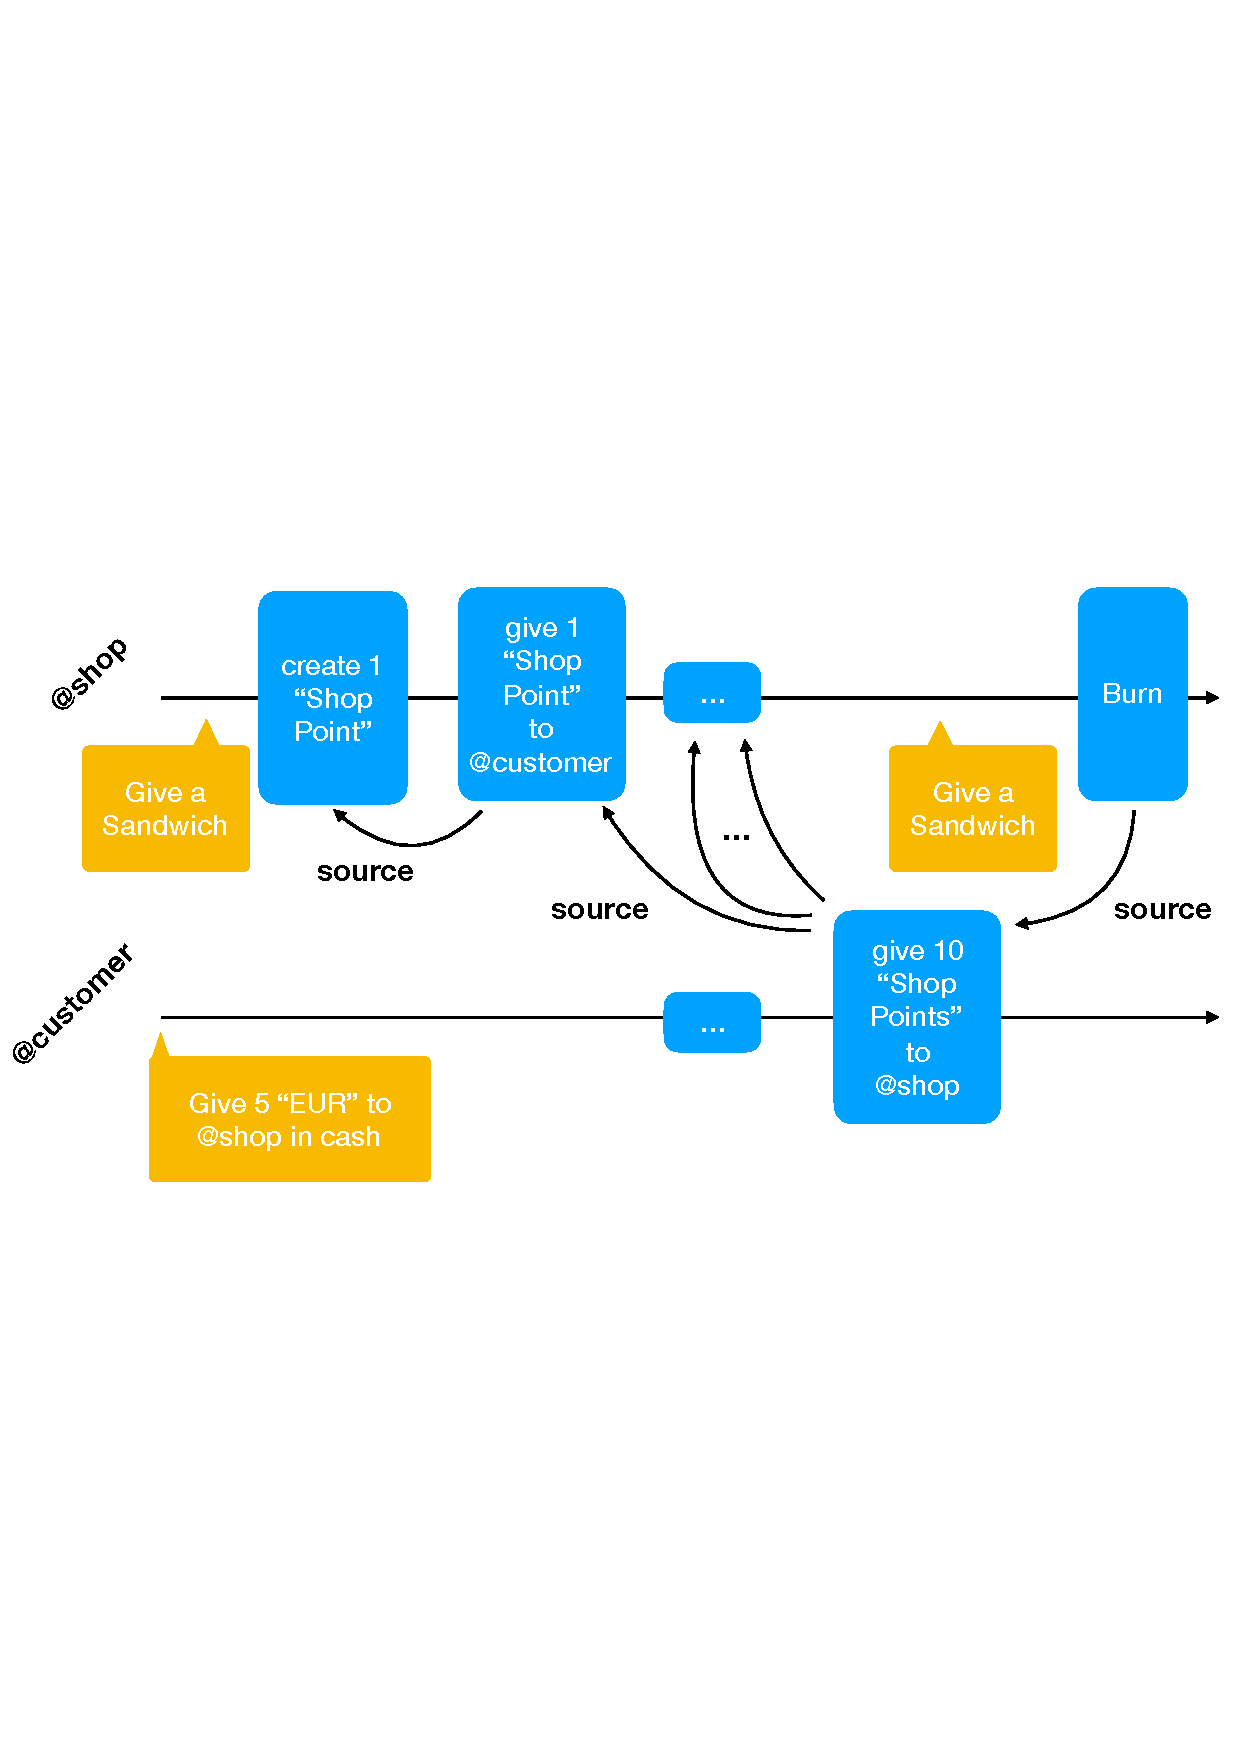
\includegraphics[width=0.40\textwidth]{./figures/example}
\caption{Example of ssb-tokens operations on SSB logs.}
\label{figure:example}
\end{figure}


\subsection{System Model}

First, we assume a fully asynchronous environment between any two nodes, i.e. that a message created by a node may take an arbitrary long time before being replicated on any other node but will eventually be replicated.\footnote{The implementation of SSB relies on partial synchrony, i.e. that most messages will be delivered before a timeout between two nodes for messages on one node to be replicated on the other, but it may take arbitrary long for any two pair of nodes to contact each other and replicate messages.}

Second, every node has an identity that corresponds to the public key of the public-private key pair that is used for signing messages, which guarantees that messages cannot be forged by nodes that don't have access to the corresponding private key. Messages are organized in an append-only log, i.e. an immutable list that can only be extended but never updated, linked to a single identity. These two properties are provided by the underlying SSB implementation (CITE Gossiping with Append-Only Logs).

Third, we assume that every node has enough storage to replicate all messages from other nodes within their community. As shown in Section~\ref{section:storage}, current common devices can store messages from Xs of users, which should be sufficient for many local applications.

Fourth, for presentation simplicity, we assume a single node and its identity correspond to a single physical person and that all activity of that person are recorded on the same log. However, implementations may allow different applications for the same person to segregate their messages in different logs without loss of generality. A log may also be updated following synchronization between different physical persons through an out-of-band protocol so that the log may represent a collective identity,  but this is out-of-scope of this paper and not covered by SSB's core operations.

\subsection{Message Format and Invariants}

\begin{table*}[t]
\centering
\caption{Message format of \textit{ssb-tokens} (JSON notation with types).}
\label{table:api}
\begin{tabular}{|l|l|} 
\hline
\textbf{Message Types}          & \textbf{Semantics}                                                                                                           \\ 
\hline
\begin{tabular}{@{}l@{}}
\texttt{\{ "type": "tokens/create", "amount": Number,}  \\
\texttt{"name": String, "unit": String, "description": SSBMsgId } \\ 
 \texttt{"smallest-unit": Number, "token-hash": String \}}
\end{tabular} ~& 
\begin{tabular}{@{}l@{}}Create \textit{amount} tokens identified by \textit{name} \\ denominated in \textit{units}, with minimum \\ 
sub-division of \textit{smallest-unit}, binding creator to \\
 promises in \textit{description}. \end{tabular}                                  \\ 
\hline
\begin{tabular}{@{}l@{}}
\texttt{\{ "type": "tokens/give", "amount": Number,} \\
\texttt{ "source": SSBMsgId, "receiver" :SSBLogId, } \\
\texttt{"token-hash": String \}}     
\end{tabular}
& Give \textit{amount} tokens from \textit{source} to \textit{receiver}.                                                                 \\ 
\hline
\begin{tabular}{@{}l@{}}
\texttt{\{ "type": "tokens/burn", "source" :SSBMsgId,} \\
\texttt{"token-hash": String \}}    
\end{tabular}             & Destroy tokens from \textit{source}.                                                                                             \\ 
\hline
\begin{tabular}{@{}l@{}}
\texttt{\{ "type": "tokens/flag", "operations": [ SSBMsgId, ... ],} \\
 \texttt{ "label": String, "token-hash": String \}} 
 \end{tabular}      &  
 \begin{tabular}{@{}l@{}}
 Assign a flag with \textit{label} on a previously \\ 
 recorded operation with \textit{ssbMsgId}. 
 \end{tabular}                             \\ 
\hline
\begin{tabular}{@{}l@{}}
\texttt{\{ "type": "tokens/unflag", "flag" :SSBMsgId \}}    
\end{tabular}
 & \begin{tabular}{@{}l@{}}Remove a previously assigned \textit{flag}.  \end{tabular}                               \\ 
\hline
%\texttt{list(tokenHash :String, owner :SSBLogId)}          & \begin{tabular}{@{}l@{}}List the current state of token, identified \\ by \textit{tokenHash}, owned by \textit{owner}.   \end{tabular}                             \\ 
%\hline
%\texttt{validate(amount :Number, src :SSBMsgId)}    & \begin{tabular}{@{}l@{}}Validate that \textit{src} has \textit{amount} \\ available and all transitive sources are valid. \end{tabular}  \\
%\hline
\end{tabular}
\end{table*}

Table~\ref{table:api} shows the core API of \textit{ssb-tokens}.\footnote{Our JavaScript implementation accepts a larger variety of inputs for convenience, including \textit{e.g.} multiple sources for giving and burning tokens which is equivalent to invoking the operations multiple times, once for each source.} The messages recorded in SSB logs have fields corresponding to the inputs of the API. In addition, all messages include an  an additional \textit{token-hash} property to make it easier to query for all messages for specific tokens, as defined by their \textit{name}, \textit{unit} and implementation-specific additional properties that uniquely describe a token. As explained in the next two sections, \textit{token-hash} makes retrieving messages required to compute the balance and validate past operations more convenient by filtering on a single property.

The \texttt{flag} and \texttt{unflag} operations are used for multiple uses. First, the creator of the tokens can \textit{cancel} tokens in circulation that have not yet been returned, to signify that the associated promise won't be honored. Second, receivers of invalid tokens, e.g. they were incorrectly formatted or the associated source did not have a sufficient remaining balance, can report the incorrect operations to exclude them from available funds locally and warn others that the operations may be incorrect. In addition, the \textit{label} field is user-defined to enable other potential user applications.



The implementation of the \texttt{create}, \texttt{flag}, and \texttt{unflag} operations is relatively straight-forward. The implementation of \texttt{give} is more involved and shown in Algorithm~\ref{algorithm:give}. The implementation of burn is similar to \textit{give} except that there is no receiver and we do not specify an amount, as the full amount of the source is burned. We forbid burning only a partial amount from a source to have partial transfers only encoded as part of \textit{give} operations.

\subsection{Computing the Balance of a Token}

\begin{algorithm}

\caption{Computing the balance of a token.}
\label{algorithm:balance}
\end{algorithm}

\subsection{Validating Past Operations}

Validation frontier: (log id, seq no, last op message id)

\begin{algorithm}

\caption{Validation of past operations.}
\label{algorithm:validation}
\end{algorithm}

\subsubsection{Double-Spending}


\begin{figure}[hb]
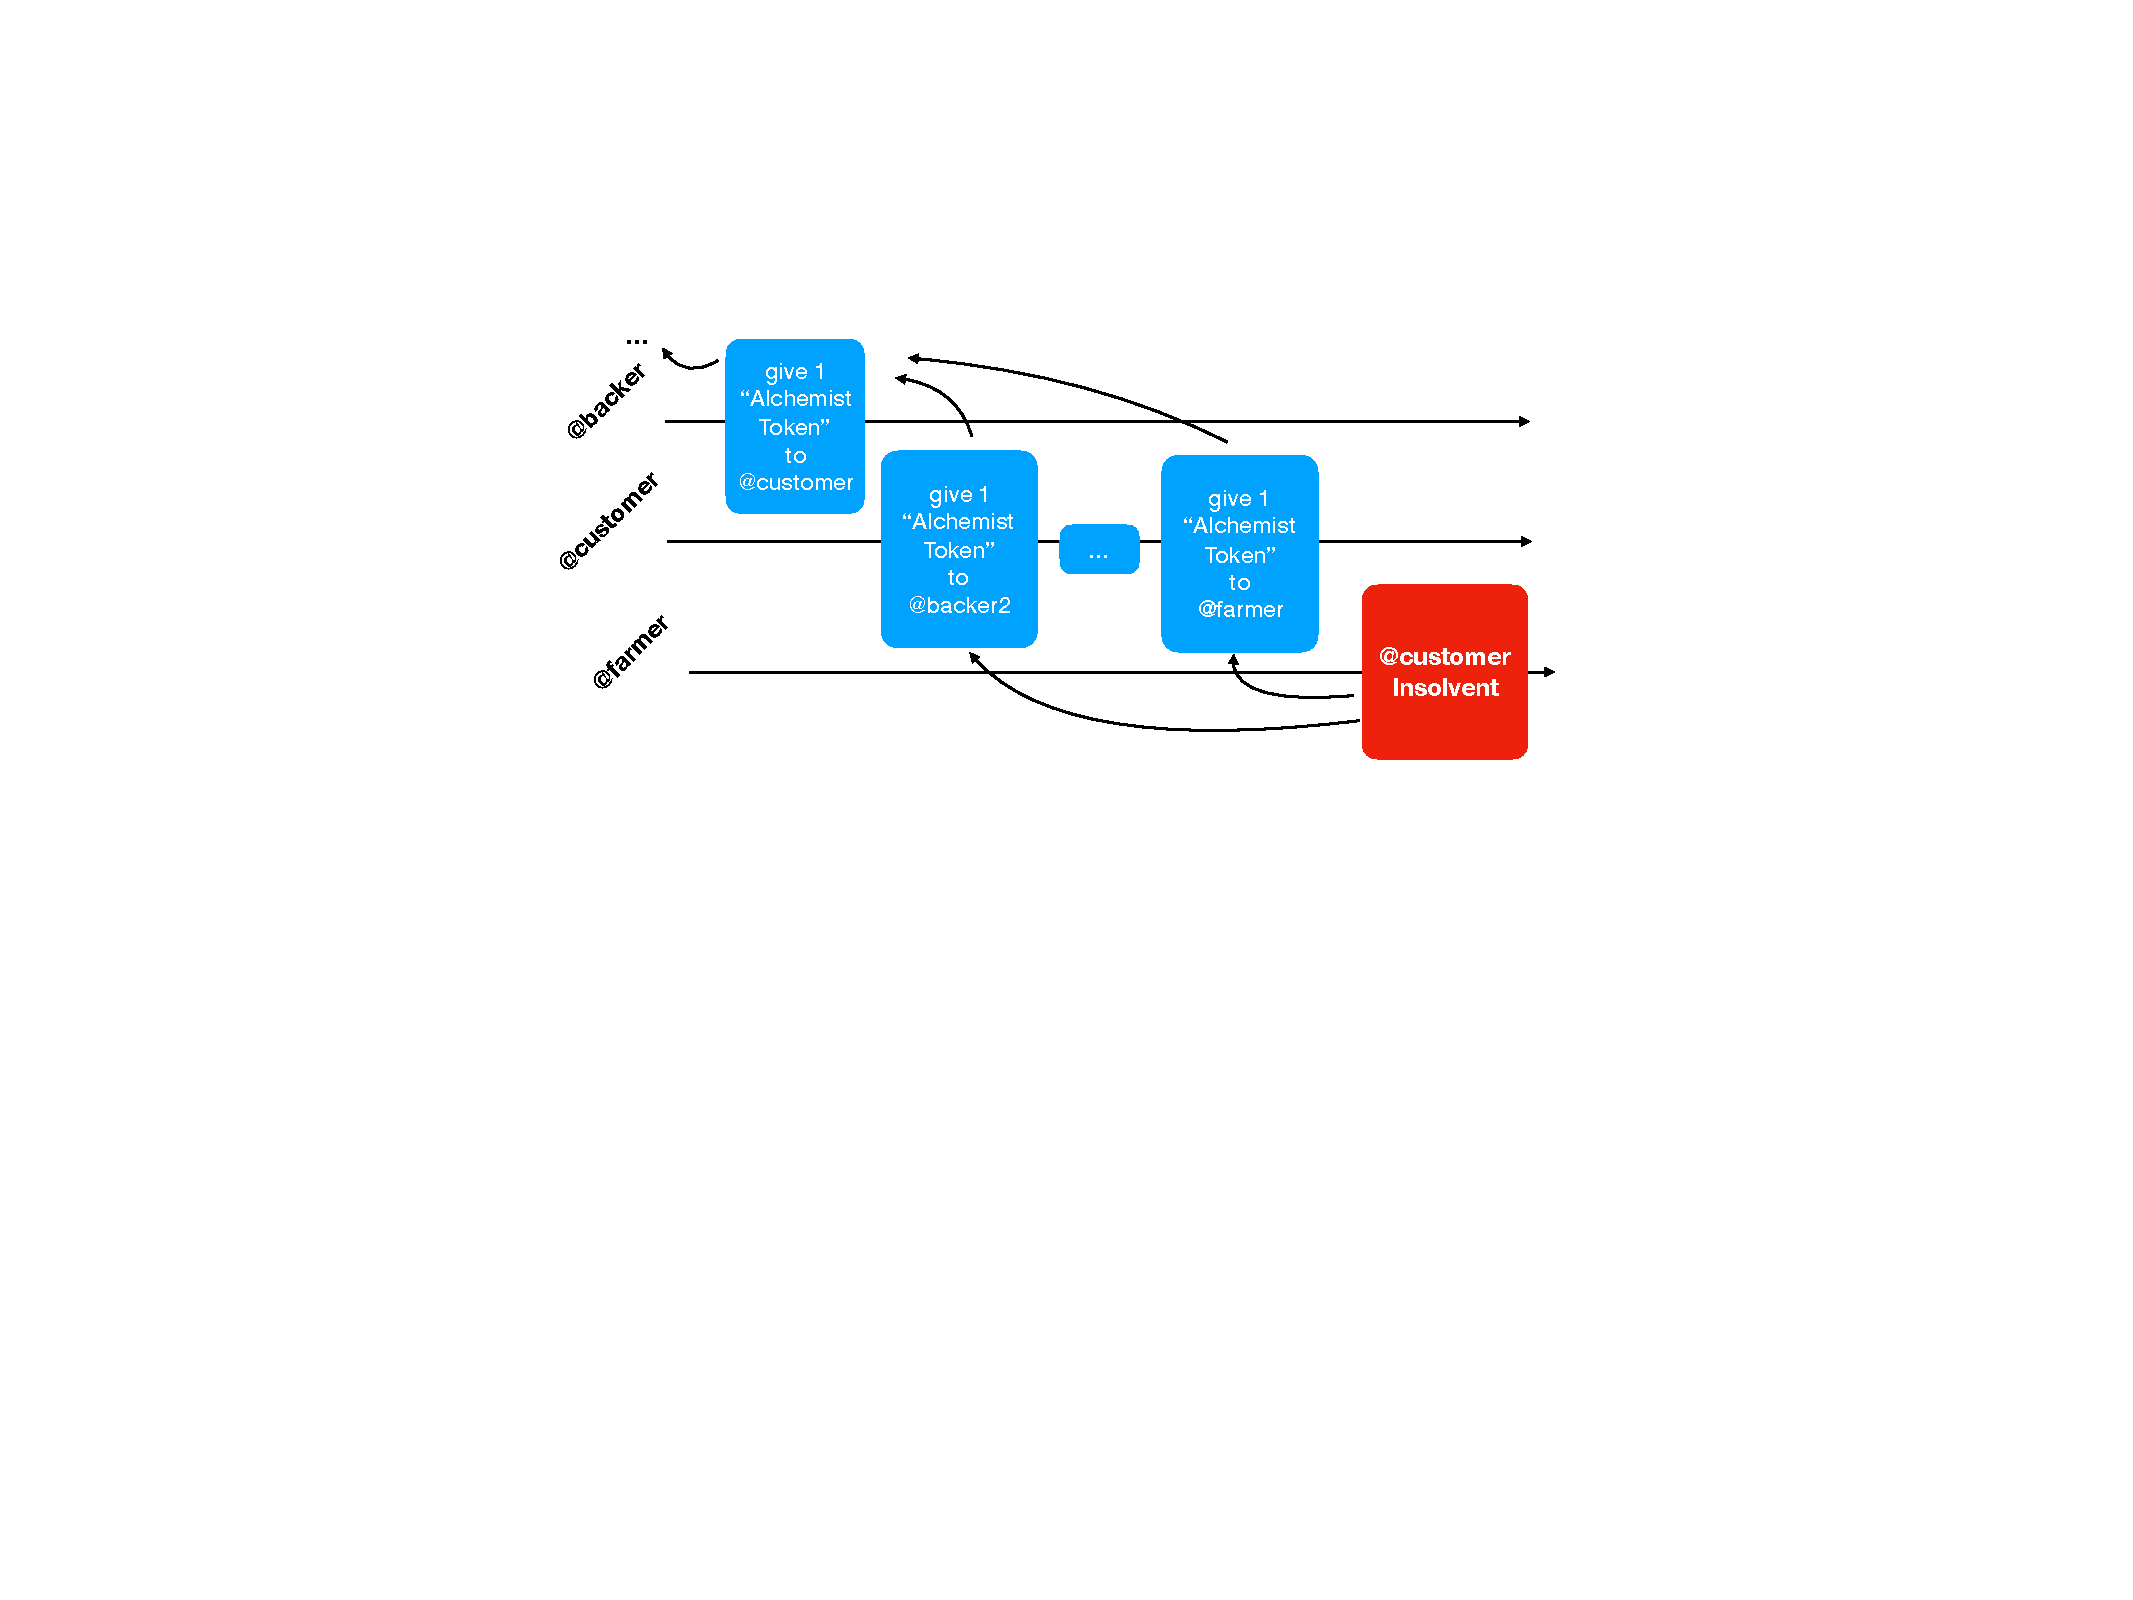
\includegraphics[width=0.45\textwidth]{figures/double-spend}
\caption{Double-Spend}
\end{figure}


\begin{figure}[hb]
\centering
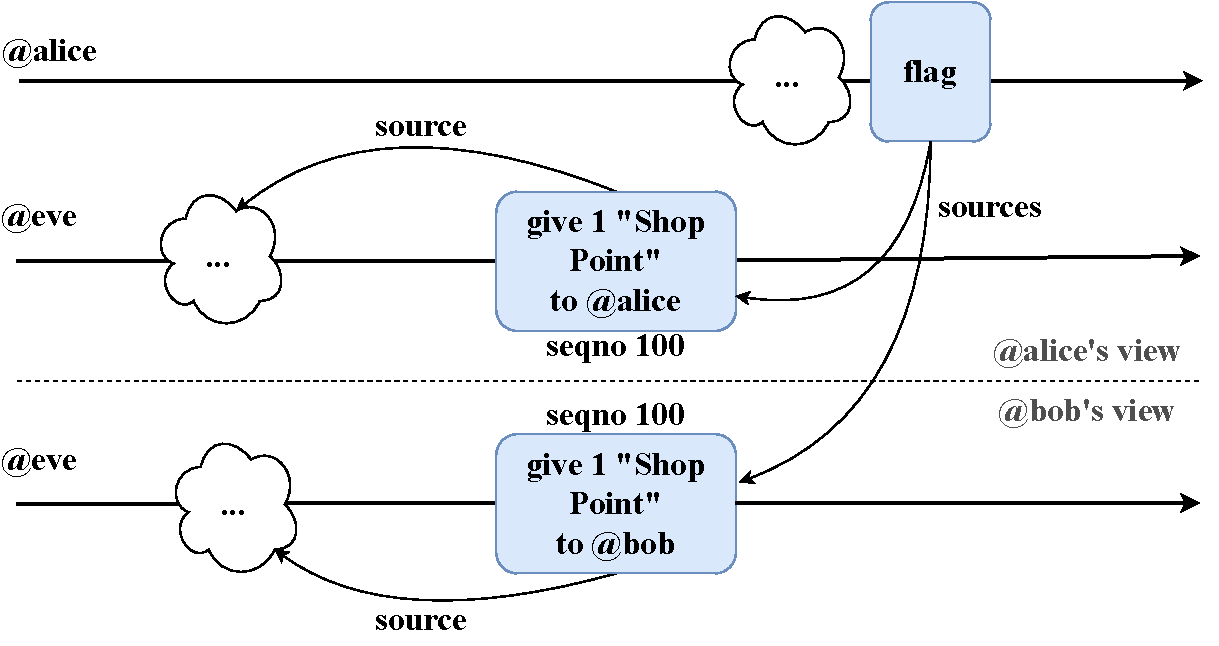
\includegraphics[width=0.45\textwidth]{figures/fork-double-spend}
\caption{Fork-based Double-Spending}
\end{figure}

\section{Additional Applications}
\label{section:applications}

\subsection{Tracking Open Source Contributions}

\subsection{Community Crowdfunding}

\subsection{Token-supported Mesh Storage and Retransmission}

A token represents a promise to store up to X bytes of messages and retransmit them to other nodes up to deadline Y.

A node pays for retransmission either with tokens it emits itself, as a reciprocal promise for retransmission of messages from other nodes, or with tokens neighbours have emitted in the past.

A node accepts to store or retransmit if a neighbour pays with tokens from itself, or with tokens from others, up to a maximum limit of X. Prior to storage a node negociate with its neighbours how much space it has available and how many tokens from different neighbours it is willing to accept.

A node may evict messages from storage earlier than deadline Y and reimburse pro rata the tokens to requester for the unused time period.

A node may assess whether another node X indeed retransmitted messages by looking for 'witness' messages that X's neighbours indeed received messages from X.

\section{Evaluation}
\label{section:evaluation}

\subsection{Setup}

Ethereum ERC dataset size

\subsection{Storage}
\label{section:storage}

bytes per transaction
transactions per user (distribution)
total storage use

Number of users supported on common devices.

\subsection{CPU}

verification time per transaction (distribution)

\section{Related Work}
\label{section:related-work}

\textbf{Producer Credits} as proposed by Paul Grignon was a major inspiration for the design of ssb-tokens. No artificial scarcity. No need for community consensus to start using them, individual economic actors can introduce their own tokens for the community they interact with.

\textbf{Local Currencies}

\textbf{Crypto-currencies and Smart-Contracts}

\textbf{TrustChain} Trust-based probabilisitic verification.


\textbf{Witness-based Validation} Crypto-currency consensus number.


\section{Conclusion and Future Work}
\label{section:conclusion}

At scale, requires an exchange service to conveniently convert one token type to another.

Integration of tokens with replication operations.






\bibliographystyle{ACM-Reference-Format}
\bibliography{social-gossip}

\appendix


\section{Open Questions}

\begin{itemize}
\item Empirical evidence (with simulation?) for scaling limit? (I am making the hypothesis that it should work 
\end{itemize}

\end{document}